\section{Evaluations} \label{sec:evals}
\subsection{The Evolution of Model Evaluation}

Assessing modern \glspl{gpm} is challenging due to their broad applicability across diverse domains. 
Unlike traditional models, which are designed for specific tasks and can be directly tested on well-defined objectives \autocite{raschka2018model}, it is impractical to evaluate \glspl{gpm} on every possible capability. As a result, many evaluations rely on structured benchmarks that measure proficiency in key areas such as mathematics, chemistry, and language understanding \autocite{tikhonov2023post}. 
However, such benchmarks often fall short in capturing open-ended problem-solving or emergent abilities that arise without explicit training for them and are sensitive to factors such as prompt phrasing and task framing \autocite{Siska2024}.

Early benchmarks primarily focused on evaluating specialized models based on their ability to predict molecular properties from molecular structures. \autocite{wu2018moleculenet} 
While useful, these evaluations largely emphasized numerical accuracy on the isolated tasks the models were fine-tuned on, without probing the more complex reasoning or generative capabilities that \glspl{gpm} aim to capture. 
Over time, this evolution expanded to exam-like problem-solving, assessing structured tasks similar to those found in academic chemistry courses. \autocite{zaki2023mascqa0, li2023camel} 
More recent efforts aim to evaluate a broader range of skills, including knowledge retrieval, logical reasoning, and even the ability to mimic human intuition when solving complex chemical problems.\autocite{feng2024sciknoweval0, mirza2024large} 
This shift highlights the need for more flexible evaluation methods that consider the specific context and nature of each task. Rather than relying solely on static benchmarks, there is a growing demand for assessments that dynamically account for the diversity of chemical tasks and the specific capabilities required to solve them---mirroring the multifaceted potential of \glspl{gpm} in chemistry. \Cref{tab:chemistry_benchmarks,fig:benchmarks} gives an overview of some benchmarks that have been used in the chemical sciences.


\begin{table}
\centering
\footnotesize
\caption{\textbf{Non-comprehensive overview of chemistry benchmarks}. Overview of chemistry benchmarks including the topics covered, the curation method (automated, using \glspl{llm}, manual), and the number of questions. We limit our scope here to benchmarks (and exclude other evaluation methods), since they constitute the most actively used and publicly available resources in the field at present.}
\label{tab:chemistry_benchmarks}
\begin{tabular}{p{3cm} p{6.9cm} p{1.2cm} p{1cm}}
\toprule
\textbf{Benchmark name} & \textbf{Overall topic} & \textbf{Curation method} & \textbf{Count} \\
\midrule
CAMEL - Chemistry \autocite{li2023camel} & General Chemistry \gls{mcq} & A, L & 20 K \\
ChemBench \autocite{mirza2024large} & General Chemistry \gls{mcq}, Reasoning & M & 2.7 K \\
ChemIQ \autocite{runcie2025assessing} & Molecule Naming, Reasoning, Reaction Generation, Spectrum Interpretation & A & 796 \\
ChemLLM \autocite{zhang2024chemllm} & Molecule Naming, Property Prediction, Reaction Prediction, Reaction Conditions Prediction, Molecule \& Reaction Generation, Molecule Description & A, L & 4.1 K \\
ChemLLMBench \autocite{guo2023large} & Molecule Naming, Property Prediction, Reaction Prediction, Reaction Conditions Prediction, Molecule \& Reaction Generation & A, L & 800 \\
LAB-Bench \autocite{laurent2024lab0bench0} & Information Extraction, Reasoning, Molecule \& Reaction Generation & A, M & 2.5 K \\
LabSafety Bench \autocite{zhou2024labsafety} & Lab Safety, Experimental Chemistry & M, L & 765 \\
LlaSMol \autocite{yu2024llasmol} & Molecule Naming, Property Prediction, Reaction Prediction, Reaction Conditions Prediction, Molecule \& Reaction Generation, Molecule Description & A, L & 3.3 M \\
MaCBench \autocite{alampara2024probing} & Multimodal Chemistry, Information Extraction, Experimental Chemistry, Material Properties \& Characterization & M & 1.2 K \\
MaScQA \autocite{zaki2023mascqa0} & Material Properties \& Characterization, Reasoning, Experimental Chemistry & A & 650 \\
MolLangBench \autocite{cai2025mollangbench} & Molecule Structure Understanding, Molecule Generation & A, M & 4 K\\
MolPuzzle \autocite{guocan} & Molecule Understanding, Spectrum Interpretation, Molecule construction & A, L, M & 23 K \\
SciAssess \autocite{cai2024sciassess0} & General Chemistry MCQ, Information Extraction, Reasoning & A, M & 2 K \\
SciKnowEval \autocite{feng2024sciknoweval0} & General Chemistry MCQ, Information Extraction, Reasoning, Lab Safety, Experimental Chemistry & A, L & 18.3 K \\
\bottomrule
\end{tabular}
\begin{tablenotes}
\footnotesize
\item \textbf{Abbreviations:} 
A: Automated methods, L: Usage of \glspl{llm}, M: Manual curation.
\end{tablenotes}
\end{table}


\begin{figure}
    \centering
    \label{fig:benchmarks}
    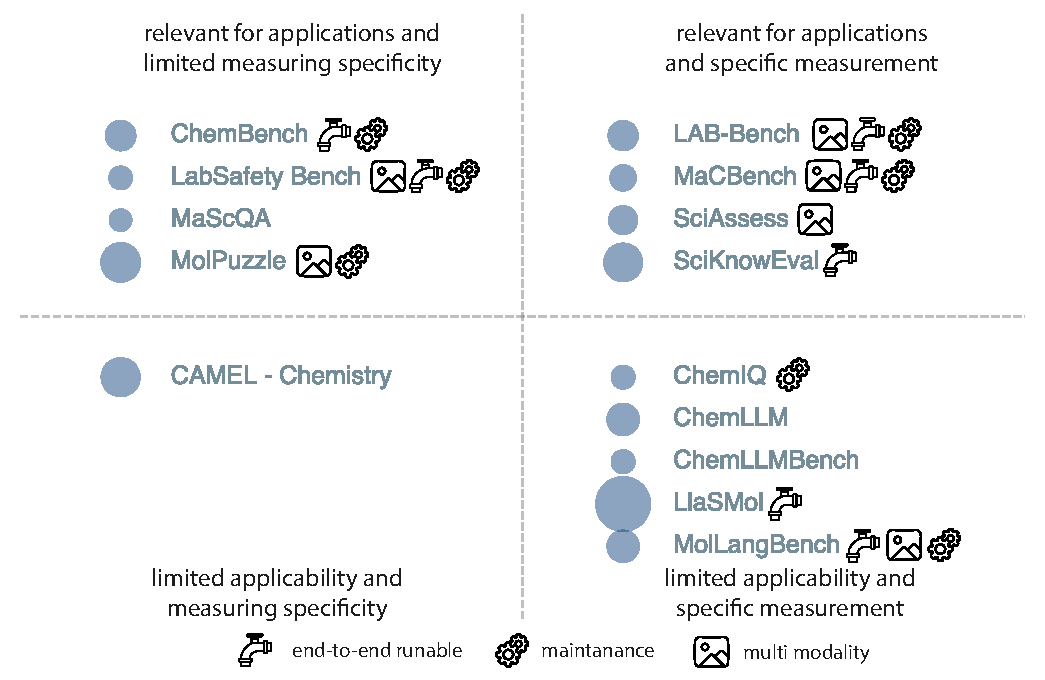
\includegraphics[width=1\textwidth]{figures/rescaled_figures/chemrev_figure8.pdf}
    \caption{\textbf{Comparison of measurement specificity and application relevance of chemistry benchmarks.} This figure presents a subjective, qualitative positioning of selected chemistry-related benchmarks along the axes of application relevance and measurement specificity (the extent to which a benchmark evaluates well-defined and objectively measurable outputs---such as physical or chemical properties---rather than more ambiguous tasks like answering general chemistry trivia or \gls{mcq}). The icons indicate whether a benchmark incorporates multimodal inputs (e.g., images or spectra), when it is actively maintained (based on GitHub activity within the past 6 months), and if it supports end-to-end evaluation via a clearly described pipeline with code provided by the authors.}
\end{figure}


\subsection{Design of Evaluations}
\label{sec:eval_design}

\paragraph{Desired Properties for Evaluations}
To meaningfully evaluate \glspl{gpm}, we must first consider what makes a good evaluation. 
Ideally, an evaluation should provide insights that translate into real-world impact, allowing comparisons between models. 
Thus, evaluation results must be stable over time and reproducible across different environments---assuming access to the same model weights or version, which is not always guaranteed when using proprietary \glspl{api}. \autocite{Ollion2024dangers}
A key challenge is so-called construct validity---ensuring that evaluations measure what truly matters rather than what is easiest to quantify. For example, asking a model to generate valid \gls{smiles} strings may test surface-level structure learning but fails to assess whether the model understands chemical reactivity or synthesis planning.
Many methods fall into the trap of assessing proxy tasks instead of meaningful competencies, which leads to misleading progress. 
However, it is important to note that proxy tasks are often chosen because measurements at higher fidelity are more expensive or time-consuming to construct. 


\paragraph{Data and Biases} The choice of what and how to measure is highly impacted by the data. 
Datasets in chemistry often differ in subtle but impactful ways: biases in chemical space coverage (e.g., overrepresented reaction types) \autocite{Jia_2019anthropogenic,Fujinuma_2022why}, variations in data fidelity (e.g., \gls{dft} vs. experimental measurements),  inconsistent underlying assumptions (e.g., simulation level or experimental conditions), and differences in task difficulty. 
These differences can distort what evaluations actually measure, making comparisons across models or tasks unreliable. \autocite{peng2024survey}
Moreover, the process of collecting or curating data itself introduces further variability, introduced by incomplete or biased coverage of the chemical space, computational constraints, or design decisions in the construction of tasks. 
As such, evaluations must be built using transparent, well-documented construction protocols, with clearly stated scope and limitations.


\paragraph{Scoring Mechanism} 

\begin{figure}
    \centering
    \label{fig:scoring}
    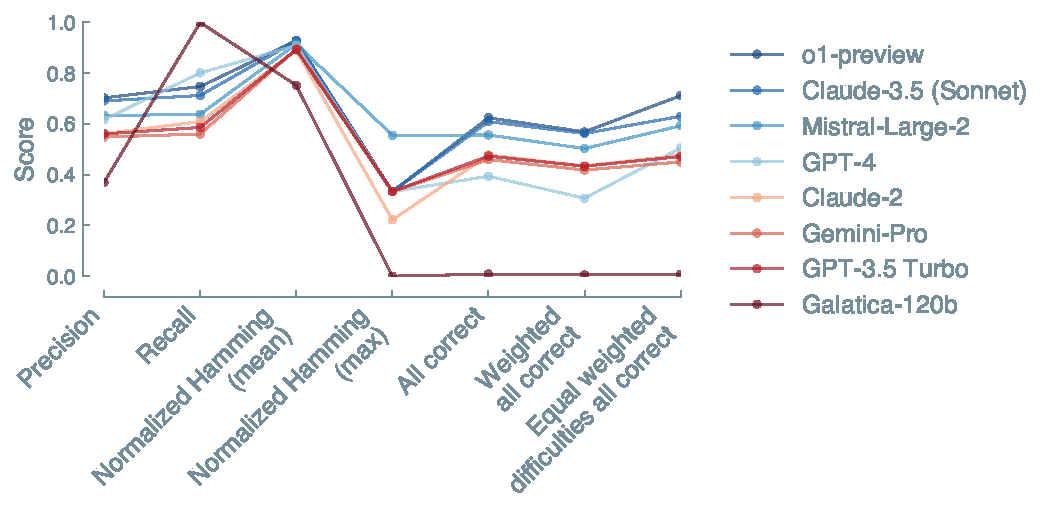
\includegraphics[width=1\textwidth]{figures/final_figures/chembench_scoring.pdf}
    \caption{\textbf{\modelname{ChemBench} \autocite{mirza2024large} rankings based on different scoring metrics}: All metrics are a sum, weighted sum, or maximum values over all \glspl{mcq}. The weighted sums are calculated by taking the manually rated difficulty (basic, immediate, advanced) of the question into account. For equal weighting, all categories are weighted equally, regardless of the number of questions. The metric \enquote{all correct} is a binary metric indicating if a given answer is completely correct. For normalized Hamming (max), the normalized maximum value of the Hamming loss of each model was taken. We find that the ranking of models changes if we change the metric, or even just the aggregation---showcasing the importance of proper and transparent evaluation design.}
\end{figure}

The way model performance is scored has a direct impact on how results are interpreted and compared. 
Leaderboards and summary statistics often shape which models are considered state-of-the-art, making even small design choices in scoring, such as metric selection, aggregation, or treatment of uncertainty, highly consequential (see \Cref{fig:scoring}). 
Inconsistent or poorly designed scoring can lead to misleading conclusions or unfair comparisons.
Metric selection and aggregation critically shape evaluation outcomes. 
For example, in tasks where multiple correct answers are possible different evaluation strategies yield different insights: a permissive metric may assign partial credit for each correct option selected, while a stricter \enquote{all-or-nothing} metric only gives credit if the full set of correct choices is identified without any mistakes. The former captures varying levels of performance, while the latter enforces a binary pass or fail threshold. Aggregation strategies, such as task averaging or difficulty-based weighting, further influence the overall score and can substantially shift model rankings. 

\paragraph{Statistical significance and uncertainty estimation} Statistical significance and uncertainty estimation are essential for drawing robust conclusions. Evaluations must include a sufficient number of questions per task type to ensure statistical power, and repeated runs (e.g., different seeds or sampling variations) are needed to report confidence intervals or error bars. \autocite{tikhonov2023post} 
While this is feasible for automated, large-scale benchmarks, it becomes significantly more challenging in resource-intensive settings such as real-world deployment studies (e.g., testing a model in a wet-lab setting), where replicability and scale are limited.

\paragraph{Reproducibility and Reporting} Without clear and consistent documentation, even well-designed evaluations risk being misunderstood or unreproducible. 
To ensure that results are interpretable, verifiable, and extensible, every step of the evaluation process should be clearly specified, from prompt formulation and data pre-processing to metric selection and aggregation. 
Standardized evaluation protocols, careful tracking of environmental variables (e.g., hardware, model version, and sampling settings such as the inference temperature for \glspl{llm}), and consistent version control (documenting the exact version of the used model) are essential to avoid unintentional variation across runs. 
Additionally, communicating limitations and design decisions openly can help the broader community understand the scope and reliability of the reported results. 
\textcite{alampara2025lessons} proposed evaluation cards as a structured format to transparently report all relevant details of an evaluation, including design choices, assumptions, and known limitations, making it easier for others to interpret, reproduce, and build upon the results.


\subsection{Evaluation Methodologies}
\label{sec:eval_methods}
\paragraph{Representational vs.\ Pragmatic Evaluations}
It is useful to think of evaluations in \gls{ml} as living on a spectrum from representational to pragmatic. 
Representational evaluations focus on measuring concepts that exist in the real world. For instance, one might ask how well a model predicts a physically significant quantity like the band gap of a material or the yield of a chemical reaction. In contrast, in pragmatic evaluations, the concept we measure is defined by the evaluation procedure itself. A well-known example of this is IQ tests. The IQ is not a physical property that exists in the world independent of the test. It is rather defined by the measurement procedure. 
In the practice of evaluating \gls{ml} models, this includes tasks like answering \gls{mcq} or completing structured benchmarks, where meaning emerges primarily through performance comparison. Such evaluations are essential for standardization and progress tracking; however, they risk creating feedback loops, as models may end up optimized for benchmark success rather than real-world usefulness, thereby reinforcing narrow objectives or biases.\autocite{alampara2025lessons, skalse2022defining}

\paragraph{Estimator Types} To systematically evaluate \glspl{gpm}, various methods (so-called estimators) have been developed, yet their application in chemistry remains limited.
Broadly, these approaches summarized in \Cref{fig:estimators} can be categorized into traditional benchmarks, challenges and competitions, red teaming and capability discovery, real-world deployment studies and ablation studies and systematic testing. 
Each evaluation method has its own strengths and limitations, and no single approach can comprehensively capture a model’s performance across all potential application scenarios.

\begin{figure}
    \centering
    \label{fig:estimators}
    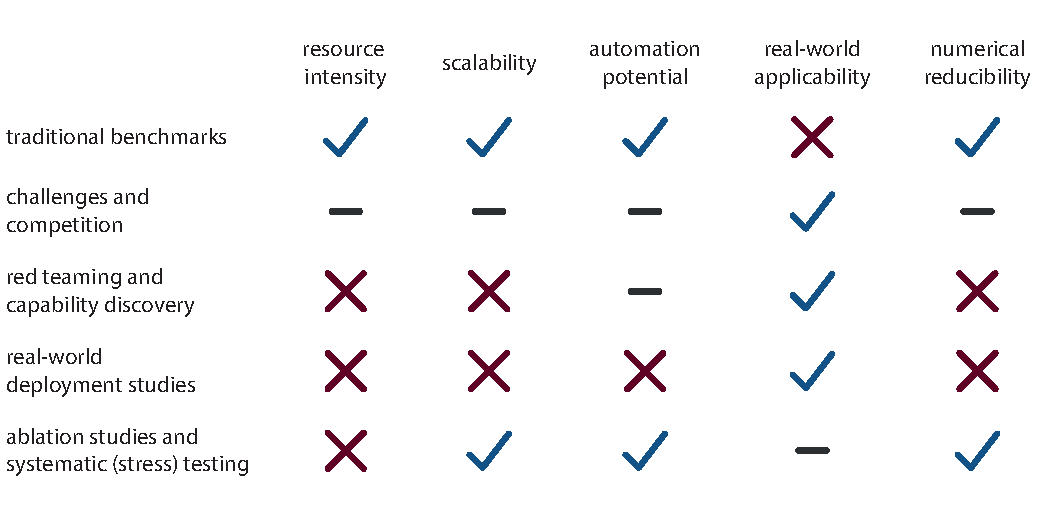
\includegraphics[width=1\textwidth]{figures/rescaled_figures/chemrev_figure10.pdf}
    \caption{\textbf{Comparison of Evaluation Methodologies}: This figure compares five common evaluation methodologies for \glspl{gpm} across the dimensions of resource intensity (required human and computational effort), scalability (ease of applying the method across tasks and models), automation potential (need for manual intervention), real-world applicability (alignment with practical use cases), and numerical reducibility (ability to express results quantitatively). Checkmarks indicate a strength in the respective dimension, crosses denote a limitation, and dashes represent a neutral position.}

\end{figure}

\paragraph{Traditional Benchmarks}\label{para:trad_benchmarks}
Traditional benchmarks can provide a fast and scalable evaluation of the models. In the context of \gls{ml}, a benchmark typically refers to a curated collection of tasks or questions alongside a defined evaluation protocol, which allows different models to be compared under the same conditions. 
Despite their advantages, summarized in \Cref{fig:estimators}, benchmarks come with several limitations. They often struggle to capture real-world impact, as they evaluate models in controlled environments that may not reflect the complexity and open-endedness of real-world applications. Current chemistry benchmarks like ChemBench\autocite{mirza2024large} and CAMEL - Chemistry\autocite{li2023camel} mostly fall on the pragmatic side of the measurement spectrum, as they are designed for comparison and decision-making rather than assessing inherent model properties. 
Classical benchmarks such as \modelname{MoleculeNet} \autocite{wu2018moleculenet} typically target molecular properties---such as solubility or binding affinity---that are experimentally measurable and representationally grounded. However, their evaluation setup, which relies on static and narrowly defined datasets, often fails to capture real-world applicability.

An additional disadvantage of traditional benchmarks is ease of overfitting, where models are optimized for high scores rather than genuine improvements. 
This problem is closely linked to data leakage---also known as test set pollution---which refers to the unintentional incorporation of test set information into the training process. Such leakage can distort performance estimates, especially when models are trained on publicly available benchmarks.\autocite{thompson2025chatbots}
This exposure increases the risk that models learn to perform well on specific benchmark questions rather than developing a deeper, more generalizable understanding of the underlying concepts, leading to an overestimation of their true capabilities. 

Several strategies have been proposed to mitigate these issues. One approach is to keep a portion of the benchmark private, preventing models from being exposed to evaluation data during training---as implemented in \modelname{LAB-Bench}, where $20\%$ of the questions are held out to safeguard against data leakage and overfitting.\autocite{laurent2024lab0bench0} 
Alternatively, some initiatives explore privacy-preserving methods or the use of trusted third parties to evaluate models on held-out data without releasing it publicly. \autocite{eleutherai2024thirdparty}
Another strategy is to regularly update benchmarks by introducing more difficult or diverse tasks over time. \autocite{jimenez2023swe} 
While this helps reduce overfitting by continually challenging models, it complicates long-term comparisons across versions and can undermine stability in performance tracking. \autocite{alampara2025lessons}

Another limitation is that most benchmarks force models to respond to every question, even when uncertain, preventing evaluation of their ability to recognize what they do not know---an essential skill in real-world settings. \modelname{LAB-Bench} addresses this by allowing models to abstain via an \enquote{insufficient information} option, enabling a more nuanced assessment that distinguishes between confident knowledge and uncertainty.


\paragraph{Challenges and Competitions}
Competitions and challenges offer a structured way to evaluate models under realistic conditions, emphasizing prospective prediction and reducing overfitting risks.\autocite{Moult2005} 
Participants typically must submit predictions for a hidden test set, enabling blind, fair evaluation that more closely mirrors real-world deployment. Unlike standard benchmarking setups, these challenges often involve tasks with temporal, external, or domain-specific novelty, making them more resistant to subtle data leakage or overfitting through test set familiarity. 
While such challenges allow for systematic and rigorous assessment of model capabilities, they also require substantial coordination and oversight by a trusted third party.

Such challenges have been rare in chemistry to date, though recent examples in areas like polymer property prediction \autocite{gang2025neurips} suggest this is beginning to change. 
More successful examples exist in related domains---most notably the \gls{caspr} competition\autocite{Moult2005} for protein structure prediction in biology, and the crystal structure prediction blind test challenge\autocite{Lommerse2000} in materials science.

\paragraph{Red Teaming and Capability Discovery} \label{para:red_teaming}
Red teaming focuses on testing models in ways that they were not explicitly designed for, often probing their weaknesses, as well as unintended and unknown behaviors. \autocite{perez2022red, ganguli2022red} 
This group of evaluations includes attempts to bypass alignment mechanisms through adversarial prompting---deliberate attempts to elicit harmful, unsafe, or hidden model outputs by manipulating the input in subtle ways---or to reveal unintended capabilities. \autocite{zhu2023prompt, kumar2023computation} 
Unlike standardized benchmarks, red teaming can reveal model abilities that remain undetected in evaluations with predefined tasks. However, a major challenge is the lack of systematic comparability. 
Results often depend on specific test strategies and are harder to quantify across models. Currently, most red teaming is conducted by human experts, making it a time-consuming process. Automated approaches are emerging to scale these evaluations, \autocite{ge2023mart0}, but in domains like chemistry, effective automation requires models to possess deep scientific knowledge, which remains a significant challenge. 

A concrete example of red teaming in chemistry was presented in the \modelname{GPT-4} Technical Report \autocite{openai2023gpt04}. 
By augmenting \modelname{GPT-4} with tools like molecule search, synthesis planning, literature retrieval, and purchasability checks, red-teamers were able to identify purchasable chemical analogs of a given compound, and even managed to have one delivered to a home address. 
While the demonstration used a benign leukemia drug, the same approach could, in principle, be applied to identify alternatives to harmful substances.\autocite{urbina2022dual}

\paragraph{Real-World Deployment Studies} 
Real-world deployment studies evaluate models in practical use settings, such as testing a \gls{gpm} in a laboratory environment. \autocite{he2020deployment}
Unlike controlled benchmarks, these studies provide insights into how models perform in dynamic, real-world conditions, capturing challenges that predefined evaluations may overlook. 
For example, a generative model might be used to suggest synthesis routes that are then tested experimentally, revealing failures due to overlooked side reactions or missing reaction feasibility. However, they come with significant drawbacks: they are highly time-consuming, and systematic comparisons between models are difficult, as real-world environments introduce variability that is hard to control. 

To date, such evaluations remain rare in the chemical sciences. 


\paragraph{Ablation Studies and Systematic Testing} 
Ablation studies analyze models by systematically isolating and testing individual components or capabilities. 
By removing or modifying specific parts of the models, the impact on performance can be evaluated, providing information on the model’s functionality and potential weaknesses. This approach can be relatively scalable and structured, allowing for thorough and reproducible assessments. Ablation studies reveal limitations and improve overall reliability by ensuring a deeper understanding of how different elements contribute to the model’s behavior. 

\textcite{alampara2024probing} conducted ablation studies to isolate the effects of scientific terminology, task complexity, and prompt guidance on model performance in multimodal chemistry tasks. 
In \modelname{MaCBench}, they showed that removing scientific terms or adding explicit guidance substantially improved model accuracy, suggesting that current models often rely on shallow heuristics rather than deep understanding. These structured ablations highlight specific failure modes and inform targeted improvements in prompt design and training strategies.

\subsection{Future Directions}

\paragraph{Emerging Evaluations Needs} To evaluate \glspl{gpm} in real-world conditions, more open-ended, multimodal, and robust approaches are needed. This is particularly evident in chemistry, where meaningful tasks often extend beyond text and require interpreting molecular structures, reaction schemes, or lab settings.
Here, vision plays a fundamental role, enabling perception and reasoning in complex environments---such as reading labels, observing color changes, or manipulating an apparatus. \autocite{Eppel2020computer}
In addition to visual cues, auditory signals---such as timer alerts or mechanical noise---can play a critical role in ensuring safety and coordination in lab environments. 
Sensorimotor input may also be relevant for simulating or guiding physical manipulation tasks, such as pipetting, adjusting equipment, or following multistep experimental procedures.


Beyond multimodality, another crucial challenge lies in evaluating open-ended scientific capabilities. 
Unlike well-defined benchmarks with fixed answers, real-world scientific inquiry is inherently open-ended.\autocite{mitchener2025bixbench0} This not only demands flexible and adaptive evaluation schemes but also raises deeper questions about what constitutes scientific understanding in generative models. 
This becomes even more important as agent-based systems (\Cref{sec:agents} gain traction---models that do not simply respond to prompts but autonomously plan, reason, and execute multistep tasks in interaction with tools, databases, and lab environments. \autocite{cao2024agents, mandal2024autonomous}
Simple input-output benchmarks are insufficient; instead, we need frameworks that can track progress in dynamic, goal-driven settings, where multiple valid solutions may exist. 

In parallel to capability assessments, the evaluation of safety (see \Cref{sec:safety}) is becoming increasingly important---especially as \glspl{gpm} gain access to sensitive scientific knowledge and tools.\autocite{bran2024augmenting, boiko2023autonomous} 
Current safety evaluations often rely on manual red teaming \Cref{sec:eval_methods}, which is neither scalable nor systematic. 
Future evaluation frameworks must therefore include robust, automated, and scalable safety testing pipelines, capable of detecting misuse potential and risky behaviors across modalities and contexts.\autocite{goldstein2023generative}

Moreover, evaluations should not be limited to static benchmarks.
One promising avenue could be the organization of recurring community-wide challenges, similar to established competitions in other fields (e.g., \gls{caspr}\autocite{Moult2005}). These challenges---ideally coordinated by major research consortia or national labs---can serve as shared reference points, drive innovation in evaluation design.

\paragraph{Standardization Efforts} One persistent challenge in evaluating \glspl{gpm} is the lack of common standards---whether in benchmark design, metric selection, or reporting protocols. This fragmentation makes it challenging to compare results or ensure reproducibility. 
While some degree of standardization can support transparency and cumulative progress, rigid frameworks risk constraining innovation and may conflict with the need in scientific discovery for more open-ended, adaptive evaluations. 

A more feasible path may lie in promoting transparent documentation of evaluation choices and developing meta-evaluation tools that assess the validity, coverage, and robustness of different approaches. Emerging frameworks such as \gls{irt} offer promising directions for such reflective evaluations, enabling nuanced insights beyond surface-level metrics. \autocite{schilling2025lifting}

